\newpage

\section{Durchführung}
\label{sec:Durchführung}

\begin{figure}
  \centering
  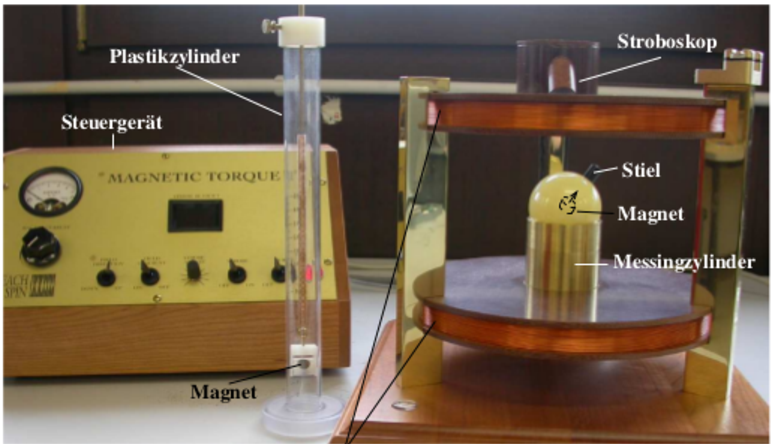
\includegraphics[width=0.8\textwidth]{content/images/bild1.pdf}
  \caption{Versuchsanordnung.}
  \label{fig:1}
\end{figure}

In eine Billardkugel ist mittig ein kleiner Stabmagnet mit
dem zu bestimmenden $\mu_{Dipol}$,welches entlang
des auf (Abb.\ref{fig:1}) zu erkennenden Stiels
gerichtet ist, eingelassen. Im Zentrum der Helmholtzspule
ist eine Vorrichtung, welche der Billardkugel erlaubt nahezu
reibungsfrei auf einem Luftkissen zu gleiten.
Die Ausmaße der verwendeten Helmholtzspule sind N = 195 Windungen mit
einem Abstand von $d = 0.138m$ und einem Spulenradius von $R = 0.109m$.
Das in (Abb.\ref{fig:1}) zu sehende Steuergerät steuert das Stroboskop, den Spulenstrom,
 Feldrichtung und -gradient.


 \subsection{Durchführung der Messung per Gravitation}
 \label{ssec:DurchGrav}

 \begin{figure}
   \centering
   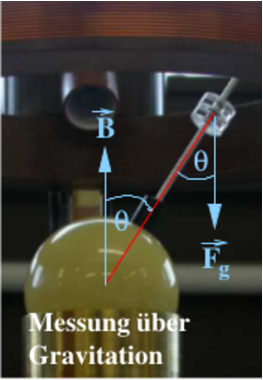
\includegraphics[width=0.3\textwidth]{content/images/bild3.pdf}
   \caption{Messung per Gravitation.}
   \label{fig:2}
 \end{figure}

In den Stiel wird eine dünne Aluminiumstange
gesteckt, an welche ein kleines Gewicht der Masse $m$ angebracht wird.
Der Abstand $r$ des Gewichtes zum Schwerpunkt der Kugel ist variabel.
Das Drehmoment der Gravitationskraft und des Magnetfeldes sind entgegengesetzt.
Zur Messung wird das Luftkissen aktiviert so, dass die Kugel möglichst
reibungsfrei gelagert ist und die Aluminiumstange samt Masse an der Kugel angebracht.
Dann wird der Spulenstrom $I_/text{Spule}$ solange erhöht bis sich ein Gleichgewicht einstellt und
$r$ und $I_/text{Spule}$ notiert. Es werden 10 Messungen mit 10 verschiedenen $r$ vorgenommen.


\subsection{Durchführung der Messung per Schwingungsdauer}
\label{ssec:DurchSchw}
